% !TeX encoding = UTF-8
% !TEX root = ./presentation.tex
\section{Referencial Teórico}
   \subsection{{\it Field-Programmable Logic Device} (FPGA) e Recursos}
      %\frame{\centering \bf \Huge \color{beamerCinza} \textit{Field-Programmable Logic Device}}
      % uso de fpga no mundo
      
      \begin{frame}{\textit{Field-Programmable Logic Device} (FPGA)}
         \begin{figure}[h] \centering
            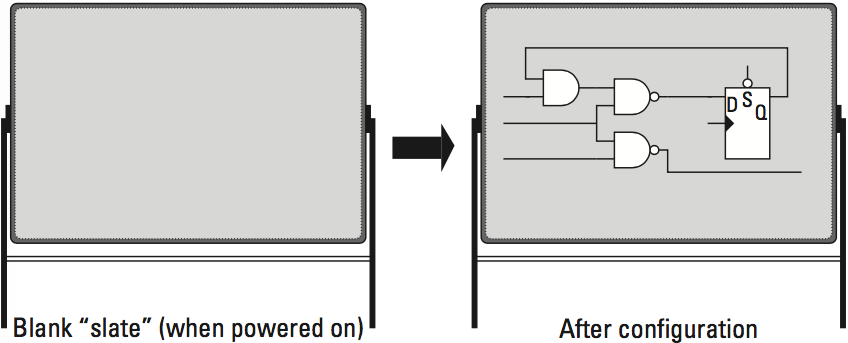
\includegraphics[width=1\textwidth]{img/rt-board.png}
            \caption{Ilustração em alto nível do funcionamento interno do FPGA. Fonte: \cite{Sass2010}.}
         \end{figure}
         \pdfnote{explicar titulo}
         \pdfnote{pode ser configurados facilmente}
         \pdfnote{linguagem ainda complexa}
      \end{frame}
   
      \begin{frame}{\textit{Field-Programmable Logic Device} (FPGA)} \vspace{-1.3em}
         \begin{figure}[h] \centering
            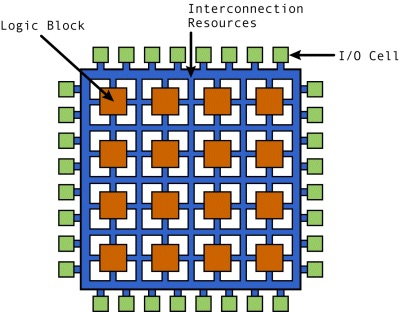
\includegraphics[width=0.75\textwidth]{img/rt-arch_fpga.jpg}
            \caption{Exemplo da arquitetura internas de um FPGA. Fonte: \url{http://www.eetimes.com/document.asp?doc_id=1274496}. Acesso: 30/05/2017.}
         \end{figure}
         \pdfnote{Tornando-o um dos (CI) MAIS densos existente.}
      \end{frame}
      
      \begin{frame}{\textit{Field-Programmable Logic Device} (FPGA)}{Introdução} \vspace{-1em}
         \begin{itemize}
            \setlength{\itemsep}{1.5em}
            \item FPGAs eram utilizados unicamente na protitipação ASIC.
            
            \item Mas com a \textbf{elevação do custo} de pesquisa, \design, desenvolvimento e teste de um novo produto
            \begin{itemize}\setlength{\itemsep}{0.5em}
               \item Interessou-se na utilização de FPGAs \cite{Mei2000};
               \item Vantagens em termos de flexibilidade de projeto.
            \end{itemize}
            
            \item Entretanto \cite{Sass2010}
            \begin{itemize}\setlength{\itemsep}{0.5em}
               \item + Configurar um \hardware\ reconfigurável é uma tarefa fácil graças às ferramentas disponíveis hoje;
               
               \item - \textbf{criar um \design\ de \hardware\ inicial não é}.
            \end{itemize}
            
         \end{itemize}
      \end{frame}
   
   
      \begin{frame}{FPGA + Processadores}{\textit{Hard} e \textit{Software Cores} \cite{Plessl2003}} \vspace{-1em} 
         \begin{itemize}
            \setlength{\itemsep}{0.5em}
            \item \textbf{\textit{Hard Core}:} \core\ dedicado;
            \item \textbf{\textit{Soft Core}:} sintetizado e mapeado no FPGA com seus recursos lógicos. 
         \end{itemize}
      
         \begin{figure}[h] \centering
            \vspace{-8pt}
            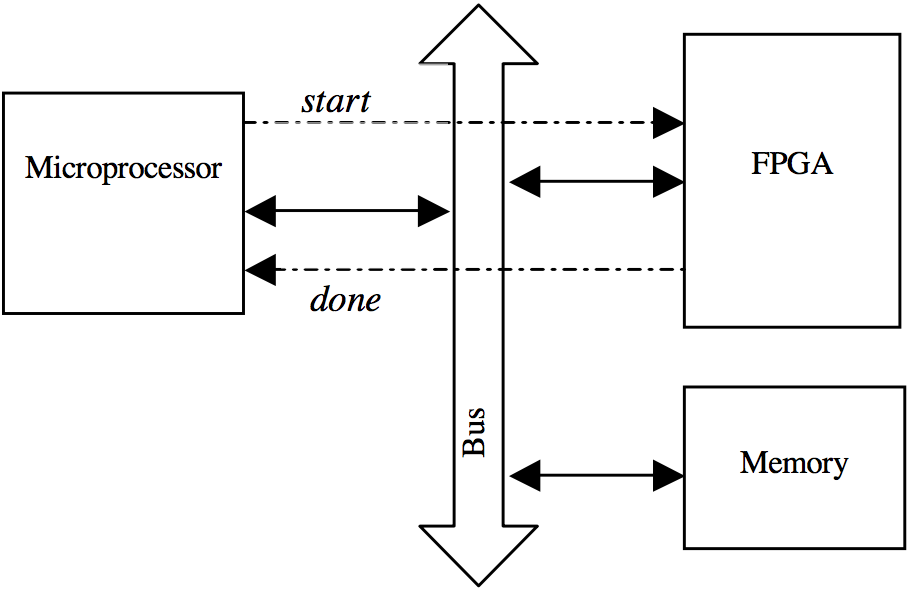
\includegraphics[width=0.7\textwidth]{img/into-soc.png}
            \caption{Visão geral de um SoC FPGA.}
            \label{fig:rb-soc}
         \end{figure}
      
         \pdfnote{HC: um pedaço de CI dentro (ou não) de um FPGA}
         \pdfnote{SC: é obtido por meio de \design\ e sintetização na placa }
         \pdfnote{vantags:}
         \pdfnote{usar todos recursos, máxima performance}
         \pdfnote{permite a extensão da arquitetura}
         \pdfnote{-> HDL}
      \end{frame}
   
      \begin{frame}{\textit{Hardware Description Language} (HDL)} \vspace{-1em}
         \begin{itemize}
            \setlength{\itemsep}{1.0em}
            \item \textbf{Classes de linguagens} de computação usados para \textbf{descrever formalmente um circuito eletrônico}.
            \begin{itemize}
               \item Pois possui detalhação altíssima do \hardware.
            \end{itemize} 
            
            \item Descreve o \cite{Sass2010}
            
            \begin{itemize}
               \item \textbf{Comportamento temporal}; ou a 
               \item \textbf{Estrutura de circuito espacial} de um sistema eletrônico.
            \end{itemize}
         
            \item Vantagens \cite{Smith1998}. 
            \begin{itemize}
               \item Pode-se \textbf{alterar} o código HDL, \textbf{e sintetizar no mesmo dispositivo} para testar;
               \item \textbf{Quantas vezes forem necessárias}, \textbf{sem custo adicional}.
            \end{itemize}
            
            \item Desvantagem
            \begin{itemize}
               \item - \textbf{Nível elevado de complexidade} de programação  \cite{Choi2016};
               \item + Existe outras linguagens disponíveis para uso \cite{Sass2010}. 
            \end{itemize}
         \end{itemize}
      \end{frame}
   
   
      \begin{frame}{\textit{High-Level Synthesis} (HLS)} \vspace{-1em}
         \begin{itemize}
            \setlength{\itemsep}{0.9em}
            \item Sintetizam códigos de alto nível para HDLs \cite{Choi2016} \cite{Trevett2008}
            \begin{itemize}
               \setlength{\itemsep}{0.2em}
               \item \textbf{Reduzir} os longos ciclos do \textbf{processo de \design}\ de \hardware; e ainda
               \item Traz \textbf{melhoria em performance e eficiência energética};
               \item Entrega um bom HDL.
            \end{itemize}
            
               \bigskip
            
            \item LegUp High-Level Synthesis
            \begin{itemize}
               \setlength{\itemsep}{0.2em}
               \item \textbf{Entrada:} código padrão \textit{C};
               \item \textbf{Saída:} compilação para dispositivos FPGA \cite{Canis2011};
               \item \textbf{Pode gerar:} \textit{hard} e \textit{soft cores};
            \end{itemize}
           
            \item OpenCL
            \begin{itemize}
               \setlength{\itemsep}{0.2em}
               \item API para \textbf{execução de programas em sistemas heterogêneos}
               \begin{itemize}
                  \item Processadores \textit{multicores}, GPUs ou outros aceleradores \cite{Shagrithaya2013, Czajkowski2012}. 
               \end{itemize}
               
               \item Nível de \textbf{paralelismo em tarefas e dados}.
               
            \end{itemize}
            \pdfnote{bib \textit{multi-threads} \textit{Pthread}, \textit{OpenMP} aceler. }
            
         \end{itemize}
      \end{frame}
   
      \begin{frame}[fragile]{}
         \begin{minted}[mathescape,
         linenos,
         fontsize=\tiny,
         framesep=2mm]{c}
void fourn(float data[], unsigned long nn[], int ndim, int isign) {
   for (ntot = 1, idim = 1; idim <= ndim; idim++) ntot *= nn[idim]; nprev = 1;
   for (idim = ndim; idim >= 1; idim--) {
      n = nn[idim]; nrem = ntot / (n * nprev);
      ip1 = nprev << 1; ip2 = ip1 * n; ip3 = ip2 * nrem; i2rev = 1;
      for (i2 = 1; i2 <= ip2; i2 += ip1) {
         if (i2 < i2rev) {
            for (i1 = i2; i1 <= i2+ip1-2; i1 += 2) {
               for (i3 = i1; i3 <= ip3; i3 += ip2) {
                  i3rev = i2rev + i3 - i2;
                  SWAP(data[i3], data[i3rev]); SWAP(data[i3+1], data[i3rev + 1]);
               }
            }
         }  ibit = ip2 >> 1;
         while (ibit >= ip1 && i2rev > ibit) { i2rev -=  ibit; ibit >>=  1; }
         i2rev += ibit;
      } ifp1 = ip1;
      while (ifp1 < ip2) {
         ifp2 = ifp1 << 1; theta = isign * 6.28318530717959 / (ifp2 / ip1);
         wtemp = sin(0.5 * theta);  wpr = -2.0 * wtemp * wtemp;
         wpi = sin(theta); wr = 1.0; wi = 0.0;
         for (i3 = 1; i3 <= ifp1; i3 += ip1) {
            for (i1 = i3; i1 <= i3 + ip1 - 2; i1 +=  2) {
               for (i2 = i1; i2 <= ip3; i2 +=  ifp2) {
                  k1 = i2; k2 = k1 + ifp1;
                  tempr = (float) wr * data[k2] - (float) wi * data[k2 + 1];
                  tempi = (float) wr * data[k2 + 1] + (float) wi * data[k2];
                  data[k2] = data[k1] - tempr;
                  data[k2 + 1] = data[k1 + 1] - tempi;
                  data[k1] += tempr; data[k1+1] += tempi;
               }
            } wr = (wtemp = wr) * wpr - wi * wpi + wr;
            wi = wi * wpr + wtemp * wpi + wi;
         } ifp1 = ifp2;
      } nprev *= n; 
   } }
         \end{minted}
\end{frame}

      \begin{frame}[fragile]{LegUp Processos}
         \begin{minted}{shell}
source ../legup.tcl
set_project CycloneV SoCKit ARM_Simple_Hybrid_System

set_accelerator_function "fourn"
\end{minted}
         \pause
         \vspace{2em}
         
         \begin{figure}
            \begin{tikzpicture}[auto, node distance=3.5 cm, >=latex']
            %\tikzstyle{block}    = [draw, rectangle, minimum height=2em, minimum width=4em, fill=red!20]
            %\tikzstyle{input}    = [coordenate]
            %\tikzstyle{output}   = [coordenate]
            %\tikzstyle{pinstyle} = [pin edge={to-,thin,black}]
            \matrix[column sep = .75cm, row sep = .375cm]{
               \node[draw, shape=rectangle, fill=red!20, visible on=<1->] (c)      {C Code}; & & \\
               &
               \node[draw, shape=rectangle, fill=red!20, visible on=<2->] (hdl)    {Generates HDL Code};&
               \node[draw, shape=rectangle, fill=red!20, visible on=<3->] (synth)  {Synthesizes it}; \\
               \node[draw, shape=rectangle, fill=red!20, visible on=<1->] (config) {Config File};& & \\
            }; 
            \draw [->, thick, visible on=<1->] (c) -- (hdl);
            \draw [->, thick, visible on=<1->] (config) -- (hdl);
            \draw [->, thick, visible on=<2->] (hdl) -- (synth);
            \end{tikzpicture}
            \caption{Processo de geração de código por meio do LegUp HLS.}
         \end{figure}
         
\end{frame}
   
      \begin{frame}[fragile]{OpenCL}
         \begin{minted}{c}
__kernel void
vectorAdd(__global const float * a,
          __global const float * b,
          __global       float * c) {
   // Indice do vetor
   int nIndex = get_global_id(0);
   
   c[nIndex] = a[nIndex] + b[nIndex];
}
         \end{minted}
\end{frame}
      
      \begin{frame}{OpenCL} \vspace{-1em}
         \begin{figure}[h] \centering
         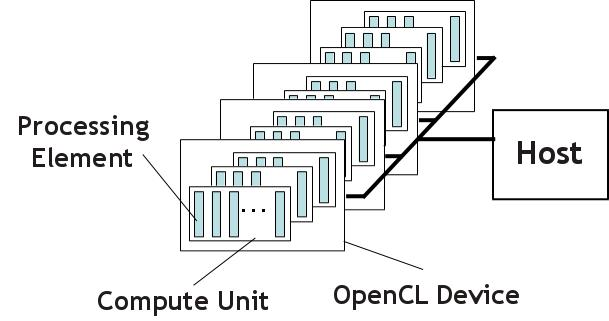
\includegraphics[width=1\textwidth]{img/opencl.jpg}
         \caption{Sistema hierárquico de um projeto em OpenCL. Fonte: \url{https://handsonopencl.github.io/} Acessado em: 07/08/2017.}
         \label{fig:opencl}
         \end{figure}
      \end{frame}


   
   \subsection{Ferramenta {\it Profile}}
   %\frame{\centering \bf \Huge \color{beamerCinza} \textit{Profile}}

      \begin{frame}{\textit{Profile}} \vspace{-1em}
         
         \begin{columns}
            \begin{column}{0.5\textwidth}
               
               \begin{figure}[h] \centering
                  \vspace{-24pt}
                  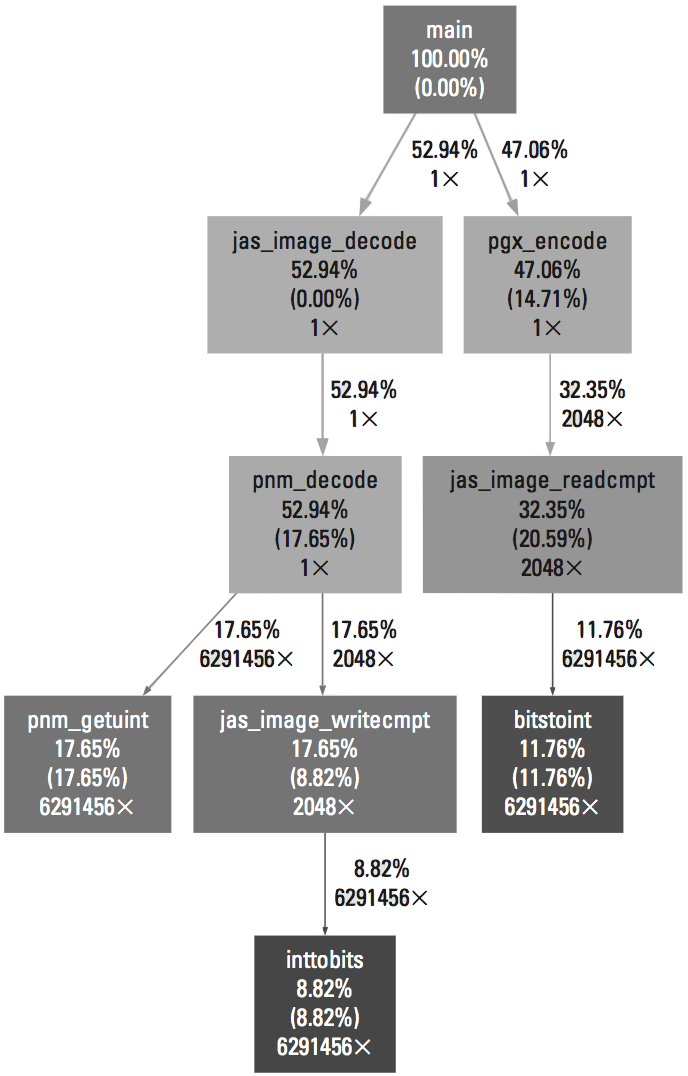
\includegraphics[width=0.8\textwidth]{img/f4-1-2.png}
                  \caption{\Profile\ da codificação de imagem em formato JPEG. Fonte: \cite{Sass2010}.}
               \end{figure}
            \end{column}
            \begin{column}{0.5\textwidth}
               \vspace{-1cm}
               \begin{itemize}
                  \item Procedimento da ferramenta
                  \begin{enumerate}
                     \setlength{\itemsep}{0.8em}
                     \item \textbf{Realiza-se interrupções periódica} no programa; e
                     \item Amostra o seu \textit{program counter}.
                     
                     \item Utiliza-se de um histograma para contar o endereço particular;
                     
                     \item \textbf{Calcula a fração aproximada do tempo} total de execução \textbf{gasto em suas partes}. 
                  \end{enumerate}
               \end{itemize}
            
            \end{column}
         \end{columns}
         \pdfnote{OLHAR OS PARENTESES (\%)}
         \pdfnote{coletar info em tempo de execução.}
         \pdfnote{soft entrada, mensura-se seu tempo.}
         
      \end{frame}


   \subsection{Sistemas Computacionais Wearables}
      %\frame{\centering \bf \Huge \color{beamerCinza} \textit{Sistemas Computacionais \Wearables}}

      \begin{frame}{\Wearables} \vspace{-1em}
         \begin{itemize} \setlength{\itemsep}{1.4em}
            \item Definição
            \begin{itemize} \setlength{\itemsep}{0.4em}
               \item Subconjunto de componentes;
               \item Possibilidade de ter recursos sensoriais e escaneamentos;
               \item Requer serviço autônomo, contínuo, em um longo período de tempo.
               \item Integrar-se ao sistema corporal;
               \item Expandindo suas capacidades;
               \item \textbf{Ou seja, são embutidos inseridos em ambiente \mobile\ de seus usuários, não exercendo a mesma atividade} \cite{Plessl2003}. 
            \end{itemize}
         
            %\item Acesso constante, conveniente, portátil e principalmente \textit{hands-free}.
            
            \item Em 2015, foi previsto um total de 6,5 bi de dispositivos ativamente conectados \cite{RobvanderMeulen2015}
            \begin{itemize} \setlength{\itemsep}{0.4em}
               \item Cerca de 20\% da população possui pelo menos um dispositivo sendo que 10\% utiliza-o todos os dias \cite{lee2016information};
               \item \textbf{Tendência:} Superar dispositivos manuais.
            \end{itemize}
            
         \end{itemize}
         \pdfnote{+ integração entre tecnologia e s.humano}
      \end{frame}  
     
      
      \begin{frame} {\Wearables}{Algumas Definições Científicas} \vspace{-1em}
         % Introdução histórica e geral
         \begin{block}{Segundo \cite{Amorim2017}:} 
            Com a possibilidade de ter um computador acoplado ao corpo, \textbf{proporciona ao usuário um nível de informações} contextualizadas \textbf{dentro de um ambiente interativo}.
         \end{block}
            
            \bigskip
      
         \begin{block}{Segundo \cite{Gemperle1998}:} 
            Dispositivo que possui sua `\textit{wearability}'. Este definido como a \textbf{interação entre o corpo humano e o objeto \textit{wearable} estendendo ao corpo em movimento}.
         \end{block}
      
      \end{frame}
   
      \begin{frame}{\Wearables}{Situação Exemplo} \vspace{-1em}
         \begin{columns}
            \begin{column}{0.6\textwidth}
               \begin{figure}[h] \centering
                  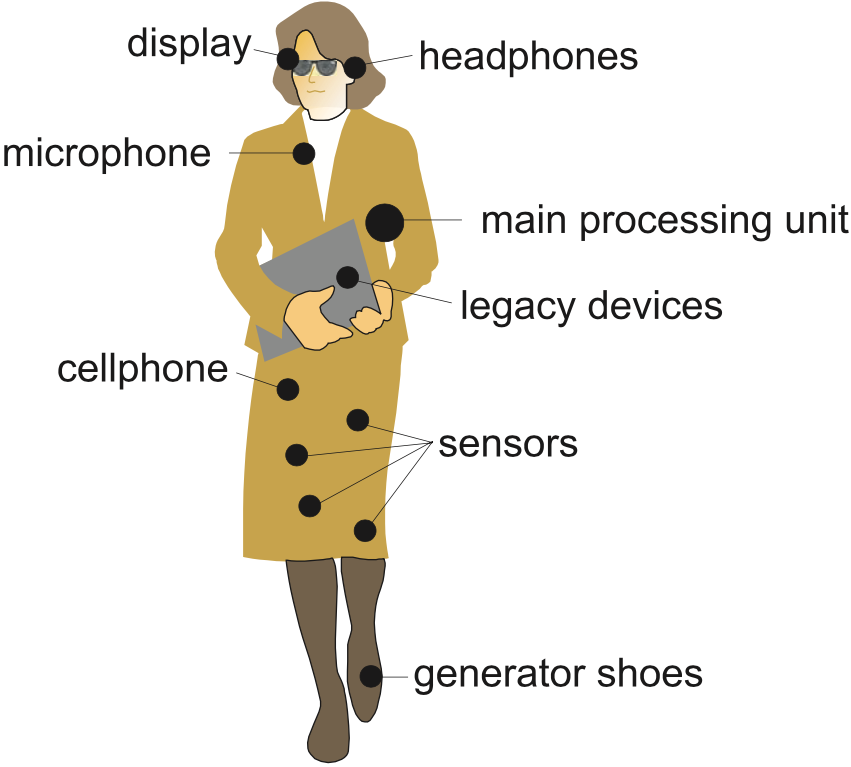
\includegraphics[width=1\textwidth]{img/into-wearable2.png}
                  \caption{Exemplificação de alguns dispositivos \wearables. Fonte: \cite{Plessl2003}.}
                  \label{fig:into-wearable}
               \end{figure}
            \end{column}
            \begin{column}{0.4\textwidth}
               \begin{itemize}
                  \item 
                  Distribuição espacial dos módulos pelo corpo;
                  
                  \item Comunicação:
                  \begin{itemize}
                     \setlength{\itemsep}{1.5em}
                     \item Deve ser avaliada energeticamente \cite{Kymissis1998}.
                     \item \textbf{Pode ser mista, sendo a predominância sem-fio pela mobilidade} \cite{Plessl2003}.
                  \end{itemize}
               \end{itemize}
               
            \end{column}
         \end{columns}
         
      \end{frame}
      
      
         % Característica de um dispositivo wearable
         \begin{frame}{Características de um \Wearable} \vspace{-1em}
            \begin{itemize} \setlength{\itemsep}{1.5em}
               \item Caracteriza-se um \wearable\ acordando \textbf{às suas funcionalidades e requisitos de \hardware}\ \cite{Delabrida2016, Amorim2017}.
               
               \item Sendo essas:
                
               \begin{itemize}
                  \setlength{\itemsep}{0.5em}
                  \item Soluções em \hardware\ \textbf{compartilham uma arq. e org. interna} de recursos comum.
                  
                  \item Também podem ser expandidos às \textbf{características de OS}.
                  
               \end{itemize}
            \end{itemize}
      
            \begin{figure}[h] \centering
               \vspace{-5pt}
               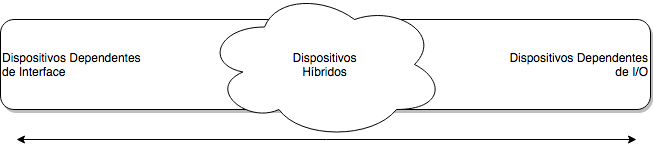
\includegraphics[width=0.9\textwidth]{img/rt-gradiente.png}
               %\vspace{-10pt}
               \caption{Classificação de \wearables. Fonte: Adaptado de \cite{Amorim2017}.}
            \end{figure}
         \end{frame}
      
      \begin{frame}{\Wearable}{Sistemas Operacionais} \vspace{-1em}
            
         \begin{itemize} \setlength{\itemsep}{1.5em}
            \item São comumente \textbf{focado em um único tipo de seguimento} de produto
            \begin{itemize}
               \item Como os \textit{smartwatches}.
            \end{itemize}
            
            \item Vantagens
            \begin{itemize}
               \item Proporcionam aos desenvolvedores um
               \begin{itemize}
                  \item Meio para sua aplicação final; além de
                  \item Produto de alta qualidade.
               \end{itemize}
            \end{itemize}
            
            \item Desvantagens
            \begin{itemize}
               \item Atualmente não existe \textbf{nenhum sistema que satisfaça todos os requisitos} de todas as classificações \cite{Amorim2017}.
            \end{itemize}
         \end{itemize}
      \end{frame}
      
      
      \begin{frame}{\Wearables}{Características a serem Consideradas no \Design} \vspace{-1em}
         
         \begin{itemize}
            \setlength{\itemsep}{0.9em}
            \item \textbf{Performance de multi-nós:} 
            \begin{itemize} \setlength{\itemsep}{0.4em}
               \item \textbf{Tarefas baixa demanda computacional ou nem restrições de tempo rigorosa}: Requer uma performance base fixa;
               
               \item Consideração de restrições de \textbf{tempo-real}.
            \end{itemize}
            
            \item \textbf{Gasto energético consciente:} 
            \begin{itemize} \setlength{\itemsep}{0.4em}
               \item Manter-se ativo e funcional num certo período de tempo;
               \item Gerenciamento do gasto de energia.
               
            \end{itemize}
            
            \item \textbf{Flexibilidade:}
            \begin{itemize} \setlength{\itemsep}{0.4em}
               \item Útil em situações altamente dinâmicas.
               \begin{itemize}
                  \item Pode variar de acordo com as escolhas do usuário ou também com o contexto e local utilizado;
                  \item Trocas de roupa.
               \end{itemize}
               \item Critérios: confiabilidade, disponibilidade e itens dependentes de sua forma como volume e peso.
            \end{itemize}
         \end{itemize}
      \end{frame}
      
      
      \begin{frame}{\Wearable\ + FPGA}{Justificativa  \cite{Plessl2003}} \vspace{-1em}
         \begin{itemize}
            \setlength{\itemsep}{1.6em}
            \item \Wearables\ necessitam
            \begin{itemize}
               \setlength{\itemsep}{0.8em}
               
               \item \textbf{Requisitos de alta performance e consumo de energia consciente:} demandam um sistema computacional econômico;
               
               \item \textbf{Requisitos flexíveis:} demanda um sistema de computação programável de propósito geral.
            \end{itemize}
         
            \item Ao utilizar de um \hardware\ reconfigurável nos permite alcançar
            \begin{itemize}
               \item \textbf{Alto processamento};
               \item \textbf{Com maior eficiência energética} comparando com processadores para computação intensiva em tempo real;
               \item Isso, junto com a disponibilidade de circuito reconfigurável para síntese.
            \end{itemize}
         \end{itemize}
      \end{frame}
